\documentclass[conference]{IEEEtran}
\usepackage{cite}
\usepackage{amsmath,amssymb}
\usepackage{graphicx}
\usepackage{booktabs}
\usepackage{microtype}
\usepackage{url}
\usepackage[hidelinks]{hyperref}

% Anonymous by default. main-camera-ready.tex enables the named author file.
\newif\ificicanonymous
\ifdefined\CameraReady
  \icicanonymousfalse
\else
  \icicanonymoustrue
\fi

\begin{document}
\raggedbottom
\title{What Pooled AUROC Hides:\\A Consequence-Stratified Pathogenicity Audit}
\ificicanonymous
  \author{\IEEEauthorblockN{Anonymous submission}}
\else
  \author{\IEEEauthorblockN{Muhammad Omar Amjad, Muhammad Ali Zain, Muhammad Ahmed, and Muhammad Awais Naeem}
\IEEEauthorblockA{University of Management and Technology, Lahore, Pakistan}
\IEEEauthorblockN{Dr. Syed Farooq Ali and Dr. Muhammad Asim Butt}
\IEEEauthorblockA{Supervisors}
}

\fi
\maketitle

\begin{abstract}
Strong pooled discrimination can hide errors within molecular consequence types. Global class balancing does not ensure adequate representation of both classes within each type. We audit a local annotation-based LightGBM pipeline using gene-component-blocked out-of-fold evaluation, consequence-specific bootstrap intervals, ablations, simple baselines, and partition controls. Pooled AUROC is 0.984, but most positive--negative pairs compare different consequences. All 68 benign frameshift variants are false positives; this failure persists in a separate unstratified sample and after removing consequence features. In-frame ranking intervals include chance, limiting conclusions for these smaller strata. First-gene and transitive-component blocking give similar pooled results, while repeated paired evaluation distinguishes partition effects from protocol variability. Excluding prior pathogenicity-predictor fields retains learned biological annotations and does not guarantee freedom from leakage. This evaluation audit shows why consequence-specific denominators, uncertainty, and targeted controls must accompany pooled ranking before biological conclusions are drawn.
\end{abstract}

\begin{IEEEkeywords}
variant pathogenicity, feature provenance, gene-component-blocked evaluation, AUROC decomposition
\end{IEEEkeywords}

\section{Introduction}

Variant pathogenicity prediction prioritizes variants for expert review, but biological evidence, labels, and partitions are interdependent. Agreement with ClinVar assertions \cite{landrum2018clinvar} is distinct from applying ACMG/AMP criteria to an individual case \cite{richards2015acmg}. A benchmark score therefore needs an explicit evidence boundary and evaluation population.

dbNSFP distributes existing predictor scores \cite{liu2020dbnsfp}, potentially importing their training history. Separately, variants from the same gene can cross a random split despite coordinate deduplication. Variant/protein overlap creates circularity \cite{grimm2015circularity}. Excluding scores and separating genes address distinct dependencies; neither guarantees useful performance within each consequence.

MX-Audit evaluates the local MAGPIE-X LightGBM pipeline, not the released MAGPIE model or an endorsed extension. We stratify errors and decompose ranking pairs, supported by ablations, simple baselines, exact-row comparators, and repeated partition controls. The question is what pooled ranking conceals, not whether a new architecture wins a benchmark.

\emph{Low-circularity} denotes the explicit feature boundary, not freedom from ascertainment, annotation dependence, or biological relatedness.

\begin{figure*}[t]
\centering
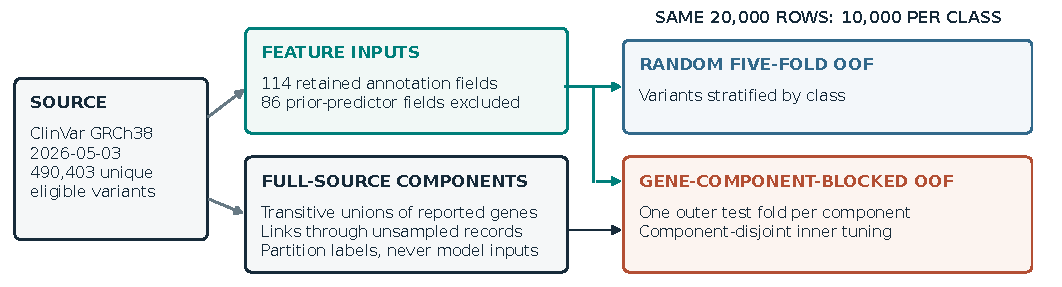
\includegraphics[width=\textwidth]{figures/experimental_design.pdf}
\caption{Full-source gene unions precede balanced sampling, preserving links through unsampled records. Each sampled row receives random and blocked OOF predictions. Inner tuning uses outer training rows only, with disjoint components in the blocked arm. Gene identifiers define partitions, never inputs.}
\label{fig:design}
\end{figure*}

\section{Related Work}

MAGPIE already excludes pathogenicity-predictor scores and uses gene-based splitting \cite{liu2024magpie,shen2024correction}; those controls are not new here. MX-Audit examines local full-source multi-gene components and consequence accounting. CADD scores genome-wide deleteriousness and supports short indels \cite{rentzsch2019cadd}; REVEL and AlphaMissense are missense-focused \cite{ioannidis2016revel,cheng2023alphamissense}. Available matched scores, rather than a tool's theoretical scope, determine our comparator coverage.

Leakage taxonomies distinguish data dependencies from test-set reuse \cite{kapoor2023leakage}. ClinGen PP3/BP4 evidence-strength calibration \cite{pejaver2022calibration} is distinct from high AUROC. We distinguish ranking, prevalence-sensitive precision--recall summaries \cite{saito2015pr}, threshold behavior, and calibration \cite{guo2017calibration}.

\section{Data and Methods}

\subsection{Data lineage and feature boundary}
The source is the 2026-05-03 ClinVar GRCh38 VCF: 490,403 unique chromosome--position--reference--alternate keys, comprising 331,524 pathogenic/likely-pathogenic and 158,879 benign/likely-benign variants after exclusion of uncertain/conflicting interpretations. These are variants, not patients. The logged annotation protocol uses ANNOVAR/refGene \cite{wang2010annovar}, \texttt{gnomAD30\_genome} \cite{karczewski2020gnomad}, and dbNSFP 4.2a. ANNOVAR's catalogue dates its dbNSFP42a build to 2021-07-10 \cite{annovar2026catalogue}; this is not the date of our ClinVar labels.

The 114 fields comprise 41 population-frequency, 30 conservation/functional, 19 consequence, 14 geometry/type, and 10 amino-acid/BLOSUM62 fields \cite{henikoff1992blosum}, including derived summaries and fitCons \cite{gulko2015fitcons}. Coordinates, identifiers, label/review metadata, and 86 prior pathogenicity-predictor fields are excluded; learned annotations remain. The feature schema is fixed from the prepared source table. Median imputation and categorical encoding are fitted within training partitions.

\subsection{Components, partitions, and model selection}
The prepared parser retains the first \texttt{GENEINFO} symbol, but 54,602 eligible variants report multiple symbols. Full-source transitive unions connect all co-reported genes before sampling: 19,927 symbols form 14,514 components across 490,403 matched eligible records. This preserves links through unsampled eligible variants. Given fixed eligibility, topology uses gene associations, not outcomes or model features.

The primary sample contains 10,000 variants per class (sampling seed 20,013), 6,024 first-gene symbols, and 5,820 components. Five-fold shuffled \texttt{StratifiedGroupKFold} (scikit-learn), seed 13, assigns each component to one outer test fold. A random stratified five-fold control uses the same rows (Fig.~\ref{fig:design}). Each row receives two OOF probabilities. This compares partition protocols, including fold composition and selection, not an isolated causal effect of leakage. The blocked estimand concerns held-out reported-gene components in this prepared population.

LightGBM 4.6.0 \cite{ke2017lightgbm} is chosen from six configurations per outer training partition, maximizing AP on the first split of a five-fold inner splitter (approximately 80/20; component-disjoint when blocked). Preprocessing and the winner are refitted on all outer training rows. Random folds select B; blocked folds select B, C, A, C, B (Table~\ref{tab:config}); estimator/inner seeds are 14--18. All fits use inverse-frequency balanced class weights and inactive row bagging. Original model reconstruction reproduced every saved primary probability within $1.2\times10^{-16}$.

\begin{table}[t]
\caption{Selected LightGBM configurations. Recovered model construction uses balanced class weights and \texttt{subsample\_freq=0}: the requested row fractions are inactive. Column sampling is active. All six candidates and constructor defaults are in the companion.}
\label{tab:config}
\centering\footnotesize
\setlength{\tabcolsep}{4pt}
\begin{tabular}{@{}lrrr@{}}
\toprule
Parameter & A & B & C \\
\midrule
Trees & 500 & 700 & 1,000 \\
Learning rate & .05 & .04 & .025 \\
Leaves / min. child samples & 31 / 20 & 31 / 30 & 63 / 40 \\
Maximum depth & not set & 6 & 8 \\
Column / requested row fraction & .90 / .90 & .95 / .95 & .90 / .80 \\
L1 / L2 & .00 / .00 & .00 / 1.00 & .05 / 1.50 \\
\bottomrule
\end{tabular}
\end{table}


\subsection{Metrics and uncertainty}
Classes use probability $\geq0.5$, an experimental cutoff, not a ClinGen evidence-strength threshold. We report ranking, threshold, and calibration metrics. AP is non-interpolated average precision, $\sum_k(R_k-R_{k-1})P_k$, historically labeled AUPRC. Ten-bin positive-class ECE weights each bin's absolute mean-probability versus positive-fraction difference by its sample fraction. No post-hoc calibration is fitted.

Random-minus-blocked differences use 1,000 paired bootstrap replicates (seed 91,013), resampling whole connected components. Percentile 95\% intervals preserve pairing and within-component dependence but condition on fitted OOF predictions: no models are retrained. They omit database/cohort uncertainty and dependence from overlapping training sets \cite{bengio2004variance}. No formal multi-metric significance claim or row-level McNemar test is made.

Ten paired OOF runs use seeds $s=13$--22, redrawing balanced samples with seed $20{,}000+s$. Both arms use the same rows; outer seed $s$ and inner/model seed $s+f$ change with fold $f$. We report per-seed differences, mean/sample SD, and exploratory two-sided sign tests, without multiplicity adjustment. Separately, ten complete 80/20 holdouts summarize the historical procedure; seed 13 is its maximum. All runs reuse one finite source population, not independent clinical cohorts.

\subsection{Evidence and consequence analyses}
Drop-one-family ablations retain blocked folds and full-model configurations, refitting without retuning. Additional controls use first-gene blocking with nested tuning, and fixed B in both random and component-blocked arms. A consequence-only logistic model uses 19 fields, training-only imputation/one-hot encoding and scaling, L2 $C=1$, balanced weights, and no tuning. An AF-only baseline ranks negative gnomAD AF, imputing missing AF with the outer-training median. Both use the blocked folds; AF scores are not probabilities. CADD PHRED, REVEL, and official GRCh38 AlphaMissense scores are matched to identical available rows per comparison, with paired component intervals.

An unstratified 20k sample contains 13,543 pathogenic variants ($\pi=0.67715$), drawn from a table with $\pi=331{,}524/490{,}403=0.67602$. It fixes B under component blocking and retains balanced training weights. Rows and selection differ from the balanced analysis; this does not isolate prevalence or class-weight effects.

Finally, we stratify the saved gene-component-blocked predictions by prepared consequence. AUROC is the fraction of correctly ordered positive--negative pairs, assigning half credit to ties. Partitioning these pairs into within- and across-consequence comparisons gives the descriptive identity
\begin{equation}
A_{\mathrm{pooled}} = w A_{\mathrm{within}} + (1-w)A_{\mathrm{across}},\quad
w=\frac{\sum_c n_c^+ n_c^-}{N^+N^-}.
\label{eq:mixture}
\end{equation}
Here $w=0.1989$ and $1-w=0.8011$ (rounded). $A_{\mathrm{within}}$ weights strata by $n_c^+n_c^-$. All ten strata contribute; groups with at least 80 rows are displayed. Stratum AUROC and paired ablation differences use 2,000 component-bootstrap replicates within each consequence (seeds $90{,}213+i$, alphabetical index $i$), rejecting draws without both classes. These are marginal, fixed-prediction intervals, not simultaneous or refitting intervals. Count-based Wilson intervals are retained as an independent-row sensitivity check at boundary error rates.

\section{Results}

The main finding is consequence heterogeneity: a high pooled AUROC coexists with zero observed frameshift specificity. We first establish the paired protocol and its variability, then examine the stratum denominators and errors that qualify the pooled result.

\subsection{Small pooled effect of gene-component blocking}
Gene-component-blocked OOF evaluation yields 0.939 accuracy, 0.879 MCC, 0.984 AUROC, and 0.981 AP (Table~\ref{tab:primary}). Every sampled variant has a held-out prediction and no component crosses a blocked split. Test folds contain 3,712--4,210 rows, with pathogenic fractions 0.470--0.523. Accuracy ranges from 0.929 to 0.945; AUROC ranges from 0.979 to 0.987. In the random control, 2,549 components span multiple test folds and therefore also connect training and test data.

\begin{table*}[t]
\caption{OOF evaluations on the same 20,000 rows and separate holdout sensitivity. Original OOF arms use nested tuning; fixed-B random equals the original random arm. AF ranking supplies no threshold/probability metrics. Each holdout tests 4,000 variants. Entries are rounded independently; differences use unrounded values. Full precision is in the companion.}
\label{tab:primary}
\centering\footnotesize
\setlength{\tabcolsep}{3pt}
\begin{tabular}{@{}lrrrrrr@{}}
\toprule
Evaluation & Accuracy & MCC & AUROC & AP & Brier & ECE \\
\midrule
Random stratified, five-fold OOF & 0.943 & 0.885 & 0.985 & 0.982 & 0.043 & 0.009 \\
Gene-component-blocked, five-fold OOF & 0.939 & 0.879 & 0.984 & 0.981 & 0.046 & 0.014 \\
First-gene blocked, nested tuning & 0.940 & 0.879 & 0.984 & 0.981 & 0.046 & 0.016 \\
Component blocked, fixed B & 0.940 & 0.880 & 0.984 & 0.981 & 0.046 & 0.011 \\
Consequence-only logistic, blocked & 0.883 & 0.781 & 0.892 & 0.916 & 0.097 & 0.002 \\
AF-only ranking, blocked & -- & -- & 0.557 & 0.515 & -- & -- \\
\midrule
Random 80/20, ten-seed mean $\pm$ SD & $0.941\pm0.004$ & $0.882\pm0.009$ & $0.984\pm0.002$ & $0.981\pm0.003$ & $0.044\pm0.003$ & $0.015\pm0.004$ \\
\bottomrule
\end{tabular}
\end{table*}


Random-minus-blocked accuracy is 0.330 percentage points (pp; 95\% component-bootstrap interval 0.107--0.550 pp): 66 additional correct classifications among 20,000 rows. Discordant counts are 219 random-only correct and 153 blocked-only correct. AUROC decreases by 0.084 pp (0.027--0.141); the AP difference is 0.086 pp ($-0.019$--0.198), with an interval crossing zero (Fig.~\ref{fig:uncertainty}). Brier score increases from 0.043 to 0.046 and ECE from 0.009 to 0.014. Differences use unrounded values, not subtraction of rounded table entries.

\begin{figure*}[t]
\centering
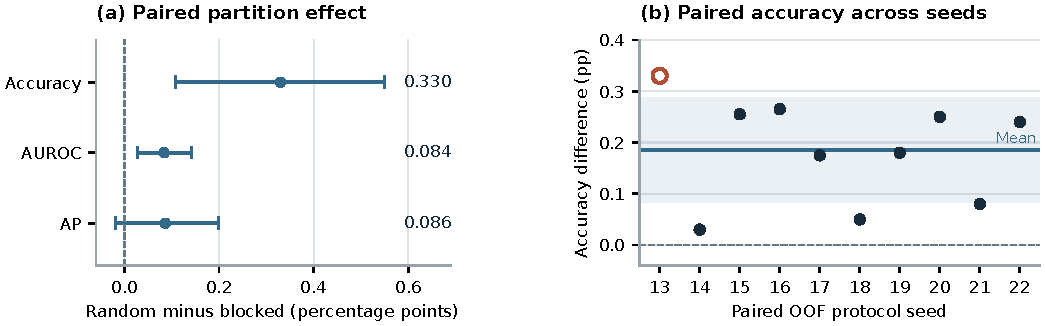
\includegraphics[width=\textwidth]{figures/split_and_seed_uncertainty.pdf}
\caption{(a) Seed-13 random-minus-blocked differences on identical OOF rows; bars: 95\% paired component-bootstrap intervals without refitting. Positive favors random splitting. (b) Accuracy differences from ten paired nested OOF runs, each refitting both arms on the same 20k sample; line: mean; shading: $\pm$ one sample SD, not a confidence interval; outline: seed 13. Units: percentage points (pp).}
\label{fig:uncertainty}
\end{figure*}

\subsection{Reproducibility across paired runs}
Across ten paired nested OOF runs, random-minus-blocked accuracy averages $0.186\pm0.102$ pp and AUROC $0.066\pm0.049$ pp (mean $\pm$ sample SD). Accuracy favors random splitting in 10/10 runs; AUROC in 9/10 (exploratory sign-test $p=0.002$ and $0.021$). The AP difference is $0.058\pm0.090$ pp, positive in 8/10 ($p=0.109$). The pooled partition effect is small and metric-dependent, with AUROC reversing in one run.

Separately, historical random-holdout accuracy is $0.94097\pm0.00441$; seed 13's 0.94675 is the maximum (range 0.93525--0.94675). The seed-13 OOF accuracy difference of 0.330 pp is smaller than this separate holdout SD of 0.441 pp. Comparing these distinct variability sources is descriptive, not a significance test; Fig.~\ref{fig:uncertainty}(b) directly repeats the paired contrast.

\subsection{Evidence dependence and comparator coverage}
Removing conservation/functional annotations reduces AUROC by 1.509 pp and MCC by 0.065. Removing population-frequency fields reduces them by 1.124 pp and 0.051. Amino-acid/BLOSUM62, consequence, and geometry/type removals produce AUROC drops of 0.247, 0.218, and 0.098 pp (Fig.~\ref{fig:evidence}). These quantify conditional predictive dependence under fixed full-model tuning.

Consequence-only logistic AUROC is 0.892 and AF-only ranking 0.557; 59.19\% of AF values are missing, limiting the latter baseline. First-gene-minus-component AUROC is $-0.006$ pp (95\% component interval $-0.060$--0.044), with no resolved incremental ranking benefit. Fixing B gives random-minus-component accuracy of 0.295 pp and AUROC of 0.085 pp (0.036--0.136), close to the nested contrast. Thus different selected configurations do not chiefly explain the seed-13 pooled effect.

\begin{table*}[t]
\caption{Exact-row comparisons, not a common leaderboard. Each score and the blocked local model (MX) use identical available rows. Coverage is relative to the 20,000-variant sample; $\pi$ is the subset's pathogenic fraction. Subsets differ between comparators, but not between models within a row.}
\label{tab:comparators}
\centering\footnotesize
\setlength{\tabcolsep}{6.2pt}
\begin{tabular}{@{}lrrrrrrr@{}}
\toprule
Score & Shared $n$ & Coverage (\%) & $\pi$ & MX AUROC & Score AUROC & MX AP & Score AP \\
\midrule
CADD & 15,015 & 75.1 & 0.368 & 0.983 & 0.967 & 0.970 & 0.946 \\
REVEL & 11,337 & 56.7 & 0.182 & 0.960 & 0.964 & 0.831 & 0.895 \\
AlphaMissense & 10,864 & 54.3 & 0.182 & 0.958 & 0.960 & 0.820 & 0.866 \\
\bottomrule
\end{tabular}
\end{table*}


On CADD's available rows, model-minus-comparator AUROC is 0.015 (95\% component interval 0.013--0.018), and AP is 0.025 (0.019--0.031). On REVEL's rows, the differences are $-0.004$ ($-0.010$--0.001) and $-0.064$ ($-0.089$--$-0.040$); on AlphaMissense's rows, $-0.002$ ($-0.007$--0.005) and $-0.046$ ($-0.072$--$-0.023$). REVEL and AlphaMissense have higher AP although their AUROC difference intervals cross zero. Both models share each comparison's prevalence, so different evaluation class fractions do not explain this AP gap. AP depends on ranking; strictly increasing recalibration preserves it. No retained comparator scores cover the 4,719 length-changing variants: an annotation-coverage gap, not evidence that CADD cannot score indels.

\subsection{What pooled performance conceals}
Global balance leaves unequal within-type class fractions (Table~\ref{tab:consequence}). Frameshift AP of 0.985 is close to its pathogenic fraction of 0.982, while AUROC is 0.563 (95\% component interval 0.491--0.633). All 68 benign frameshifts are called pathogenic; the nominal independent-row Wilson specificity interval is 0.000--0.053. In-frame deletion/insertion AUROCs are 0.490 (0.400--0.585) and 0.497 (0.342--0.643). Intervals including 0.5 indicate unresolved ranking evidence, not proof of equivalence to chance.

\begin{figure*}[t]
\centering
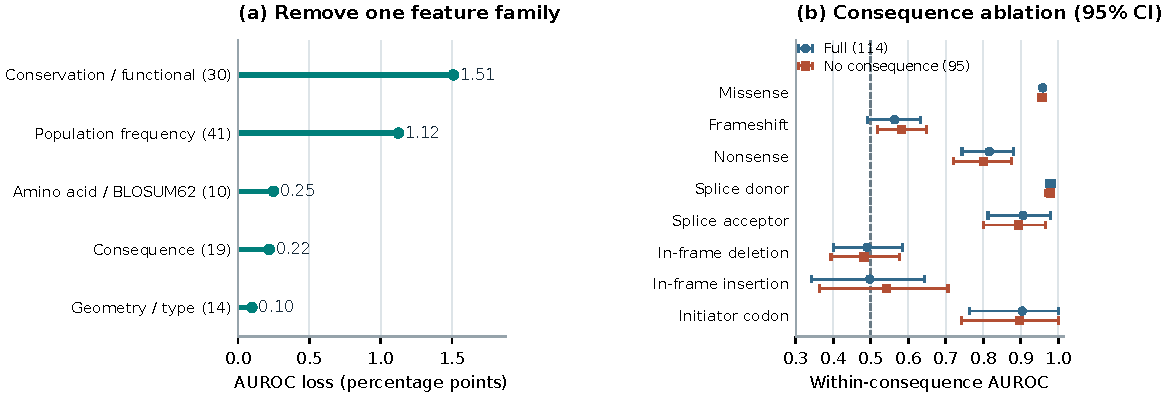
\includegraphics[width=\textwidth]{figures/evidence_and_consequences.pdf}
\caption{(a) AUROC loss after removing each feature family with fixed folds/configurations. (b) Full 114-field and consequence-drop 95-field models on identical rows: within-consequence AUROC with marginal 95\% component-bootstrap intervals (2,000 replicates, fixed predictions). The dashed line marks chance ranking. Intervals omit refitting uncertainty; paired differences are in the companion. Table~\ref{tab:consequence} supplies denominators and full-model threshold errors.}
\label{fig:evidence}
\end{figure*}

\begin{table*}[t]
\caption{Consequence-specific OOF results ($n\geq80$). P/B: pathogenic/benign including likely labels; $\pi=P/n$. Brackets: marginal 95\% component-bootstrap AUROC intervals (2,000 replicates within each stratum; fixed predictions, no refitting). Sensitivity/specificity use threshold 0.5. AP must be interpreted alongside $\pi$, particularly for frameshift and nonsense.}
\label{tab:consequence}
\centering\footnotesize
\setlength{\tabcolsep}{3.0pt}
\begin{tabular}{@{}lrrrrrrr@{}}
\toprule
Consequence & $n$ & P/B & $\pi$ & AP & AUROC [95\% CI] & Sens. & Spec. \\
\midrule
Missense & 11,614 & 2,026/9,588 & 0.174 & 0.815 & 0.958 [0.952, 0.964] & 0.742 & 0.955 \\
Frameshift & 3,856 & 3,788/68 & 0.982 & 0.985 & 0.563 [0.491, 0.633] & 1.000 & 0.000 \\
Nonsense & 2,505 & 2,450/55 & 0.978 & 0.992 & 0.816 [0.743, 0.880] & 0.996 & 0.364 \\
Splice donor & 878 & 836/42 & 0.952 & 0.999 & 0.980 [0.969, 0.989] & 0.993 & 0.619 \\
Splice acceptor & 750 & 713/37 & 0.951 & 0.987 & 0.906 [0.813, 0.979] & 0.996 & 0.486 \\
In-frame deletion & 185 & 68/117 & 0.368 & 0.402 & 0.490 [0.400, 0.585] & 0.132 & 0.932 \\
In-frame insertion & 87 & 21/66 & 0.241 & 0.295 & 0.497 [0.342, 0.643] & 0.095 & 0.970 \\
Initiator codon & 81 & 72/9 & 0.889 & 0.985 & 0.904 [0.764, 1.000] & 0.986 & 0.778 \\
\bottomrule
\end{tabular}
\end{table*}


Equation~\ref{eq:mixture} quantifies this composition effect. Of 100 million positive--negative pairs, 80.11\% cross consequence types. Their AUROC is 0.992; the within-consequence pair-weighted value is 0.952, combining to pooled 0.984. Missense supplies 97.67\% of within-consequence pairs, so this summary cannot represent rare strata uniformly. The identity describes where ranking comes from, not how much is caused by consequence features.

Removing the 19 consequence fields leaves frameshift specificity at zero. In-frame deletion sensitivity rises from 0.132 to 0.382, but specificity falls from 0.932 to 0.581 and AUROC remains near chance (0.481). This is a threshold trade-off, not recovered ranking; paired stratum ablation intervals are supplied in the companion.

\subsection{Probability and class-mix sensitivity}
The unstratified sample yields 0.981 AUROC, 0.988 AP, 0.045 Brier, and 0.022 ECE. Frameshift contains 5,124 pathogenic and 61 benign variants: specificity remains zero and AUROC is 0.452 (0.382--0.526). Missense AUROC is 0.960 (0.953--0.965); nonsense specificity is 0.316. The complete stratum results are in the companion. Thus the observed frameshift failure is not confined to the globally balanced sample, although sample composition, tuning, and weighting prevent a causal attribution to balancing.

\section{Discussion and Limitations}

\subsection{What the stratification establishes}
Global balancing leaves frameshift/nonsense predominantly pathogenic and missense predominantly benign. A model can exploit this structure without resolving difficult within-type cases. Persistence under unstratified sampling and consequence removal argues against a balancing-only or consequence-fields-only explanation, but does not identify a cause. These data cannot distinguish intrinsically poor benign-frameshift discrimination from insufficient benign training examples. Correlated annotations and transcript policy remain alternatives.

Component intervals condition on fitted scores; overlapping training folds add dependence. Boundary threshold estimates can produce degenerate bootstrap intervals, motivating the separately labeled Wilson check, which itself ignores clustering. Neither interval estimates clinical operating characteristics.

\subsection{What the partition comparison does not isolate}
The sample's 6,024 first-gene labels become 5,820 components: 204 fewer groups (3.4\%), not 204 affected variants. The incremental ranking effect is unresolved, but transitive union closes reported-gene paths through unsampled records. Protein families, homology, and shared annotation histories remain unblocked.

Fixed-B controls reduce the tuning confound, but changing partitions necessarily changes training composition. Paired seed variation and fixed-prediction intervals address distinct uncertainties; neither is external-cohort validation. Pooled OOF ranking compares scores from different fitted models, not one prospective deployed classifier.

\subsection{External validity}
Learned annotations remain; ClinVar assertions may incorporate computational evidence, and comparator training overlap is unaudited. The 2026 labels and 2021 dbNSFP generation are not historically synchronized. The recovered ANNOVAR installation reports annotation-script revision dated 2025-03-02 and table-wrapper revision dated 2022-08-02; hashes identify current files at the logged path, not proof of unchanged historical binaries. AlphaMissense's exact release remains unverified. No independent, ancestry-stratified, or prospective validation was performed. A label-temporal test needs verified first-availability dates and must disclose contemporary annotations; last-evaluated dates or file timestamps are insufficient.

\subsection{Reproducibility scope}
The \href{https://github.com/Shouwiya/MAGPIE-X-FYP/tree/conference-audit-v1.1/conference-audit}{MAGPIE-X-FYP companion (conference-audit-v1.1)} provides aggregate evidence, configurations, feature definitions, provenance hashes, verification and plotting scripts, and a prepared-input primary-training entry point. A fresh-environment author-side refit reproduced both primary nested OOF arms, including fold assignments, selected configurations, and saved probabilities. Research inputs remain necessary; source annotation and all secondary experiments are not independently reproduced by this release. Row-level variants, labels, predictions, feature values, and fitted artifacts are excluded. No DOI is claimed.

\subsection{Data and declarations}
This retrospective computational audit uses ClinVar-derived variant assertions and population annotations, with no new participant recruitment or individual patient records. It makes no claim of institutional ethics exemption. This research received no external funding. The authors declare no conflict of interest.

\section{Conclusion}
High pooled ranking does not ensure useful discrimination within variant types. Despite blocked AUROC of 0.984, benign frameshift recognition fails in both sampling analyses and after consequence-feature removal. Simple baselines, grouping controls, and stratum intervals make the result more specific without making it clinical validation. Report consequence denominators, uncertainty, and targeted controls alongside pooled metrics; independent, temporally grounded validation remains necessary before clinical use.

\bibliographystyle{IEEEtran}
\bibliography{references}
\end{document}
